% ==============================================================================
% 插曲 2：引用与反引用 (Intermezzo 2: Quote, Unquote)
% ==============================================================================

\intermezzo{插曲 2：引用与反引用}
\label{sec:intermezzo02}

列表在本书以及作为我们教学语言基石的 Racket 中都扮演着至关重要的角色。对于程序设计而言，从基本原理（first principles）理解列表是如何从 \code{cons} 和 \code{'()} 一步步构建出来的极其关键，这直接决定了我们如何系统化地编写程序。然而，在日常开发中，频繁处理长列表需要更加紧凑便捷的记法，正如第 11.1 节引入的 \code{list} 简写函数。

早在 20 世纪 50 年代末，以 Lisp 为代表的函数式语言家族就配备了一对更为强大的列表构建利器：\term{引用}（quotation）与\term{反引用}（anti-quotation / unquote）。如今许多现代编程语言都提供了类似支持（例如 PHP 的模板插值或 JavaScript 的模板字符串，都深受这一思想启发）。

本插曲将带你初步领略这种优雅强大的引用机制，并引入与引用密不可分的全新数据形式——\term{符号}（Symbol）。

\intermezzosection{引用 (Quote)}

\term{引用}（Quotation）是一种极其简练地书写长列表的语法机制。通俗地说，任何使用 \code{list} 函数构造的列表，都可以通过对列表进行“引用”以更加紧凑的方式写出。

从技术上讲，\code{quote} 是一个语法关键字，例如：\code{(quote (1 2 3))}。DrRacket 会将其直接翻译为 \code{(list 1 2 3)}。而单引号 \code{'} 则是 \code{quote} 的快捷简写：
\begin{replbox}
> '(1 2 3)
(list 1 2 3)
> '("a" "b" "c")
(list "a" "b" "c")
> '(#true "hello world" 42)
(list #true "hello world" 42)
\end{replbox}

如果说对简单列表而言，\code{'} 相比 \code{list} 只是略微减少了几个字符，那么在处理多层嵌套列表时，引用的威力便显露无遗：
\begin{replbox}
> '(("a" 1)
    ("b" 2)
    ("d" 4))
(list (list "a" 1) (list "b" 2) (list "d" 4))
\end{replbox}
只需最外层一个单引号 \code{'}，就能一举构造出任意深度的嵌套列表！

要理解引用的求值规则，可以将其想象为一个遍历表达式形状的展开函数：
\begin{itemize}
  \item 当 \code{'} 遇到原子基本数据（数字、字符串、布尔值或图像）时，它会自动消失；
  \item 当 \code{'} 位于开括号 \code{(} 前面时，它会在括号后插入 \code{list}，并将 \code{'} 递归分发给该括号内部的每一个元素。
\end{itemize}
例如：
\begin{lstlisting}[language=BSL]
'(1 2 3)        ; 等价于 (list '1 '2 '3) -> (list 1 2 3)
'(("a" 1) 3)    ; 等价于 (list '("a" 1) '3) -> (list (list "a" 1) 3)
\end{lstlisting}

\begin{exercise}{消除 quote 简写}{231}
将下列各表达式中的 \code{'} 消除，改用 \code{list} 显式表达，并进一步改写为仅使用 \code{cons} 和 \code{'()} 的版本：
\begin{enumerate}
  \item \code{'(1 "a" 2 \#false 3 "c")}
  \item \code{'()}
  \item 如下表格形状：
\begin{lstlisting}[language=BSL]
'(("alan" 1000)
  ("barb" 2000)
  ("carl" 1500))
\end{lstlisting}
\end{enumerate}
\end{exercise}

\intermezzosection{准引用与反引用 (Quasiquote and Unquote)}

你可能会问：既然引用如此方便，为什么前面的章节直到现在才介绍它？

在初学程序设计阶段，过早依赖 \code{'} 容易导致误解。使用 \code{cons} 一步步构建列表能够清晰揭示递归与归纳的本质；而简写往往隐藏了这一底层结构。此外，引用还隐藏着一个意想不到的“陷阱”。

假设你在定义区中定义了常量：
\begin{lstlisting}[language=BSL]
(define x 42)
\end{lstlisting}
若在交互区尝试运行：
\begin{replbox}
> '(40 41 x 43 44)
(list 40 41 'x 43 44)
\end{replbox}
请注意：返回的并非预期的 \code{42}，而是 \code{'x}！这里的 \code{'x} 是一个全新的数据类型——\term{符号}（Symbol）。符号是值本身，而不是代表值的变量！它与变量 \code{x} 没有任何代换关联。

同理，若执行：
\begin{replbox}
> '(1 (+ 1 1) 3)
(list 1 (list '+ 1 1) 3)
\end{replbox}
这里的 \code{'+} 只是一个符号，加法表达式根本没有被执行，而是被完整地原样引用为一个三元素嵌套子列表！

在很多时候，我们希望在引用的骨架中，\textbf{特定部分能够逃逸出引用状态，像普通代码一样被正常计算}。为此，语言引入了\term{准引用}（quasiquote，简写为反引号 \code{\`{}}）与\term{反引用}（unquote，简写为逗号 \code{, }）：
\begin{replbox}
> `(40 41 ,x 43 44)
(list 40 41 42 43 44)
> `(1 ,(+ 1 1) 3)
(list 1 2 3)
\end{replbox}

其背后的规则极其直观：反引号 \code{\`{}} 在括号内部展开，但当遇到逗号 \code{, } 时，两者相互抵消，逗号后面的表达式被当作常规代码予以求值求结果！

这一机制在\term{网页动态生成}中展现出惊人的威力。在 BSL+ 中，我们可以利用准引用模板非常直观地生成 HTML 网页数据结构（如图~\ref{fig:html_generator} 所示）。

\begin{figure}[htbp]
  \centering
  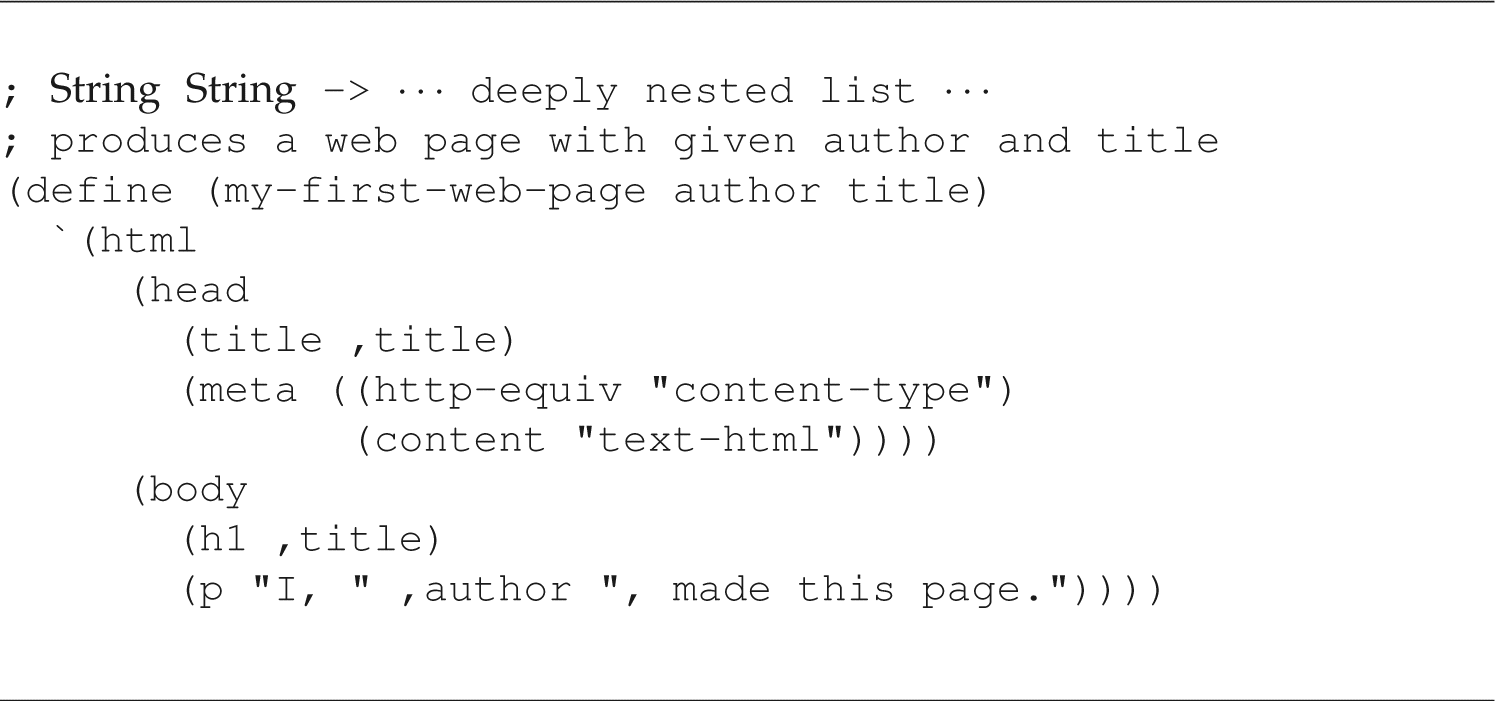
\includegraphics[width=0.85\textwidth]{images/00301.png}
  \caption{基于准引用与反引用的简易 HTML 页面生成器}
  \label{fig:html_generator}
\end{figure}

图~\ref{fig:nested_lists_webpage} 对比了该函数生成的嵌套列表与等价的标准 HTML 代码。

\begin{figure}[htbp]
  \centering
  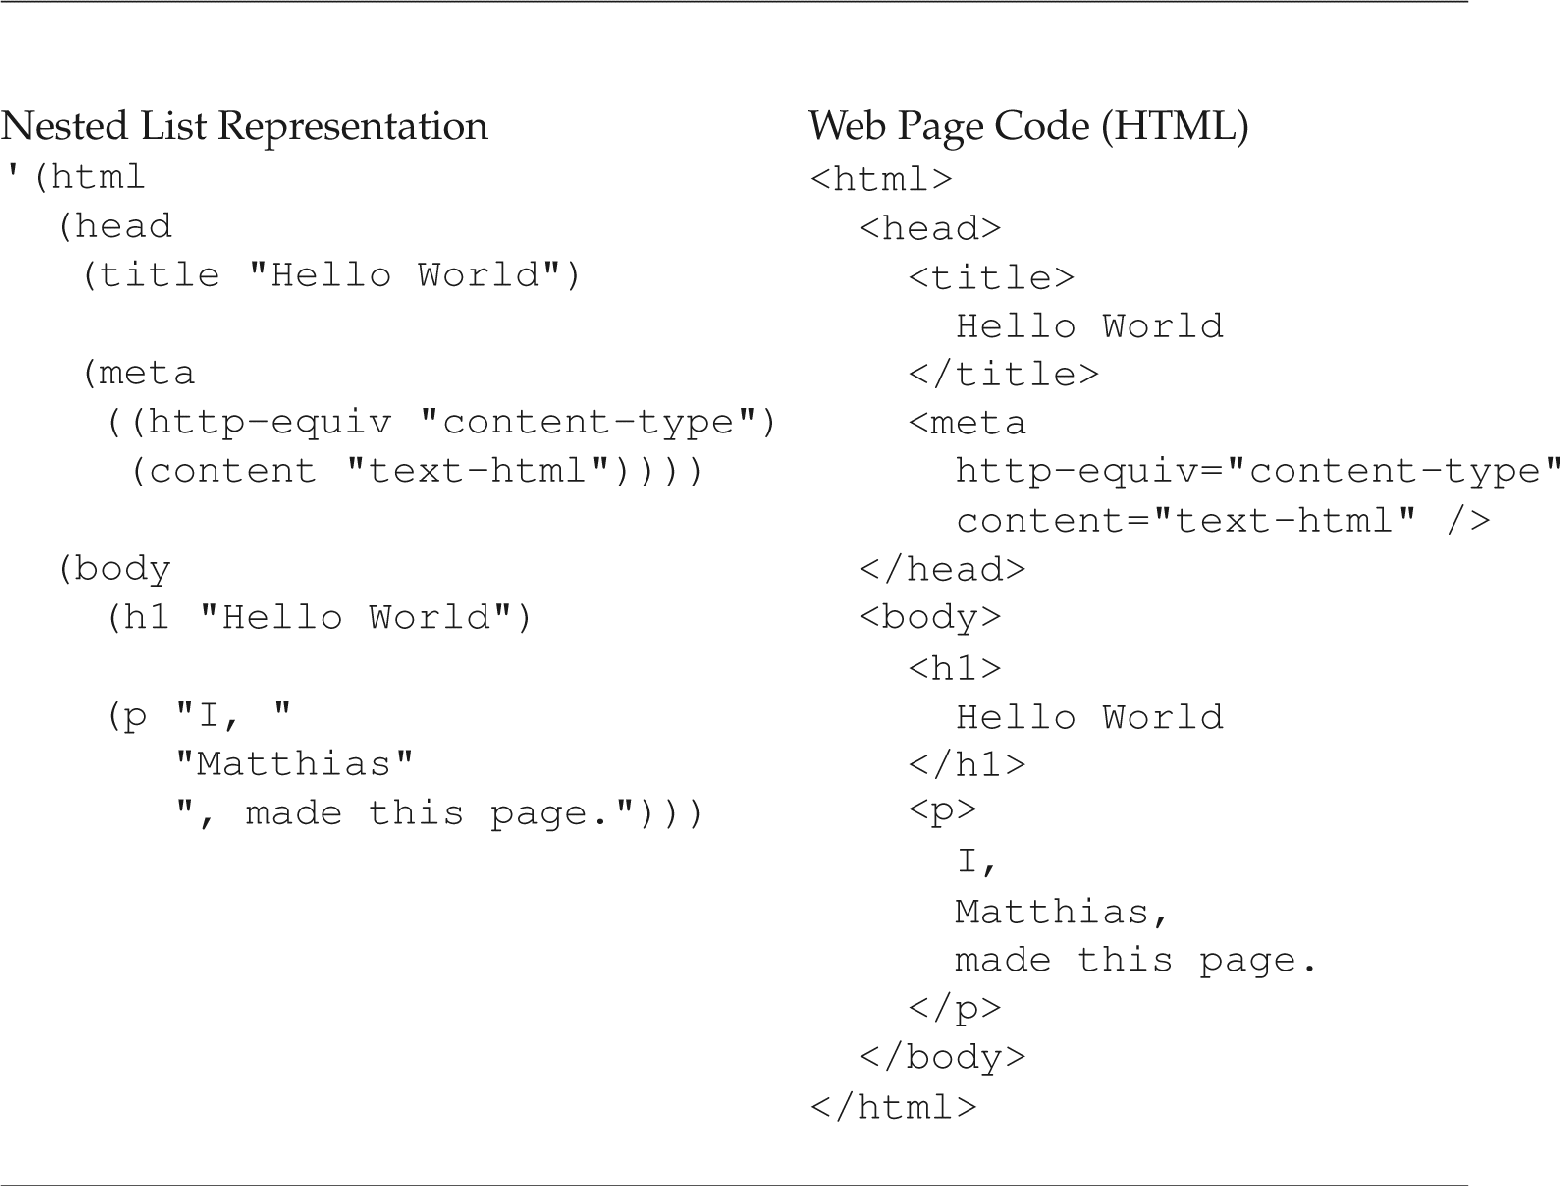
\includegraphics[width=0.85\textwidth]{images/00302.png}
  \caption{嵌套列表与对应生成的 HTML 网页源代码}
  \label{fig:nested_lists_webpage}
\end{figure}

\begin{exercise}{消除准引用与反引用}{232}
使用 \code{list} 消除下列各式中的反引号 \code{\`{}} 与逗号 \code{, }：
\begin{enumerate}
  \item \code{\`(1 "a" 2 \#false 3 "c")}
  \item 表格数据：
\begin{lstlisting}[language=BSL]
`(("alan" ,(* 2 500))
  ("barb" 2000)
  (,(string-append "carl" " , the great") 1500)
  ("dawn" 2300))
\end{lstlisting}
  \item 包含动态标题的网页结构。
\end{enumerate}
\end{exercise}

\intermezzosection{反引用拼接 (Unquote Splice)}

当子函数产生一个列表，而我们希望\textbf{将该子列表中的元素直接平铺、打散拼接到外层列表中}（而非作为一个独立的嵌套子列表）时，普通的反引用 \code{, } 就无法满足要求了：
\begin{replbox}
> `(tr ,(list "3" "4" "5"))
(list 'tr (list "3" "4" "5"))
\end{replbox}
而我们期望的结果往往是：
\begin{lstlisting}[language=BSL]
(list 'tr "3" "4" "5")
\end{lstlisting}

为此，BSL+ 提供了\term{反引用拼接}操作符 \code{,@}（unquote-splicing）：
\begin{replbox}
> `(tr ,@(list "3" "4" "5"))
(list 'tr "3" "4" "5")
\end{replbox}
它相当于把内层列表的外壳“剥开”，将其中的所有元素无缝融入外层列表！

利用 \code{,@}，我们可以极为优雅地编写函数生成任意行列尺寸的 HTML 表格：
\begin{lstlisting}[language=BSL]
; Number -> List
(define (make-cell n)
  `(td ,(number->string n)))

; List-of-numbers -> List
(define (make-row l)
  (cond
    [(empty? l) '()]
    [else (cons (make-cell (first l))
                (make-row (rest l)))]))

; List-of-numbers List-of-numbers -> List
(define (make-table row1 row2)
  `(table ((border "1"))
     (tr ,@(make-row row1))
     (tr ,@(make-row row2))))
\end{lstlisting}

\begin{exercise}{消除拼接简写}{233}
用 \code{list} 和 \code{cons} 重写包含 \code{,@} 的下列各式，并使用 \code{check-expect} 进行等价性检验：
\begin{enumerate}
  \item \code{\`(0 ,@'(1 2 3) 4)}
  \item 包含子列表拼接的表格行定义。
\end{enumerate}
\end{exercise}

\begin{exercise}{生成音乐排行榜网页 make-ranking}{234}
设计函数 \code{make-ranking}：消耗带有排名的歌曲名称列表，生成整齐美观的 HTML 网页表格展示（如图~\ref{fig:generated_webpage} 所示）。
\end{exercise}

\begin{figure}[htbp]
  \centering
  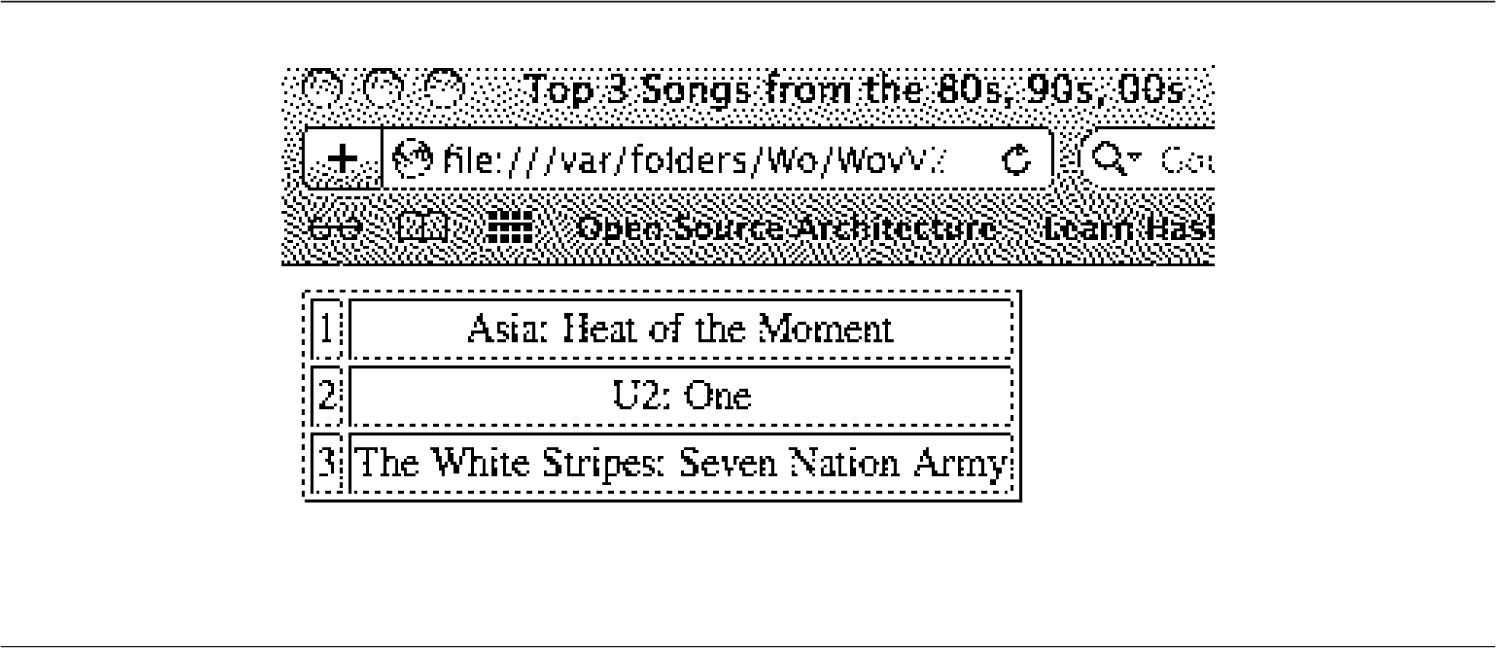
\includegraphics[width=0.75\textwidth]{images/00312.png}
  \caption{由 BSL+ 程序自动生成的动态网页效果}
  \label{fig:generated_webpage}
\end{figure}
